\documentclass{article}

\usepackage{fancyhdr} % Required for custom headers
\usepackage{lastpage} % Required to determine the last page for the footer
\usepackage{extramarks} % Required for headers and footers
\usepackage[usenames,dvipsnames]{color} % Required for custom colors
\usepackage{graphicx} % Required to insert images
\usepackage{listings} % Required for insertion of code
\usepackage{courier} % Required for the courier font
\usepackage{lipsum} % Used for inserting dummy 'Lorem ipsum' text into the template
\usepackage{amsmath}
\usepackage{amssymb}
\usepackage{mathtools, xparse}
\usepackage{booktabs}
\usepackage{bigstrut}
\usepackage{float}
\usepackage{hyperref}
\usepackage{color}
\usepackage{algorithm}
\usepackage{caption}
\captionsetup{skip=0pt}
\usepackage{algpseudocode}
\usepackage{multirow}
\usepackage{subfigure}
\usepackage{longtable}
\usepackage{supertabular}
\usepackage{biblatex}

\renewcommand*{\Rnfont}{\scshape}

\DeclarePairedDelimiter{\norm}{\lVert}{\rVert}
\DeclarePairedDelimiter\abs{\lvert}{\rvert}%

\hypersetup{
    colorlinks   = true,    % Colours links instead of ugly boxes
    urlcolor     = red,    % Colour for external hyperlinks
    linkcolor    = red,    % Colour of internal links
    citecolor    = red      % Colour of citations
}
% Margins
\topmargin=-0.45in
\evensidemargin=0in
\oddsidemargin=0in
\textwidth=6.5in
\textheight=9.0in
\headsep=0.25in

\linespread{1.1} % Line spacing

% Set up the header and footer
\pagestyle{fancy}
\lhead{\hmwkAuthorName} % Top left header
\rhead{\hmwkClass\ : \hmwkID} % Top center head
%\rhead{\firstxmark} % Top right header
\lfoot{\lastxmark} % Bottom left footer
\cfoot{} % Bottom center footer
\rfoot{Page\ \thepage\ of\ \protect\pageref*{LastPage}} % Bottom right footer
\renewcommand\headrulewidth{0.4pt} % Size of the header rule
\renewcommand\footrulewidth{0.4pt} % Size of the footer rule
\renewcommand{\subsectionmark}[1]{\markboth{#1}{}}
\setlength\parindent{0pt} % Removes all indentation from paragraphs

%----------------------------------------------------------------------------------------
%	CODE INCLUSION CONFIGURATION
%----------------------------------------------------------------------------------------

\definecolor{MyDarkGreen}{rgb}{0.0,0.4,0.0} % This is the color used for comments
\lstloadlanguages{Perl} % Load Perl syntax for listings, for a list of other languages supported see: ftp://ftp.tex.ac.uk/tex-archive/macros/latex/contrib/listings/listings.pdf
\lstset{language=Perl, % Use Perl in this example
    frame=single, % Single frame around code
    basicstyle=\small\ttfamily, % Use small true type font
    keywordstyle=[1]\color{Blue}\bf, % Perl functions bold and blue
    keywordstyle=[2]\color{Purple}, % Perl function arguments purple
    keywordstyle=[3]\color{Blue}\underbar, % Custom functions underlined and blue
    identifierstyle=, % Nothing special about identifiers                                         
    commentstyle=\usefont{T1}{pcr}{m}{sl}\color{MyDarkGreen}\small, % Comments small dark green courier font
    stringstyle=\color{Purple}, % Strings are purple
    showstringspaces=false, % Don't put marks in string spaces
    tabsize=5, % 5 spaces per tab
    %
    % Put standard Perl functions not included in the default language here
    morekeywords={rand},
    %
    % Put Perl function parameters here
    morekeywords=[2]{on, off, interp},
    %
    % Put user defined functions here
    morekeywords=[3]{test},
    %
    morecomment=[l][\color{Blue}]{...}, % Line continuation (...) like blue comment
    numbers=left, % Line numbers on left
    firstnumber=1, % Line numbers start with line 1
    numberstyle=\tiny\color{Blue}, % Line numbers are blue and small
    stepnumber=5 % Line numbers go in steps of 5
}

% Creates a new command to include a perl script, the first parameter is the filename of the script (without .pl), the second parameter is the caption
\newcommand{\perlscript}[2]{
    \begin{itemize}
        \item[]\lstinputlisting[caption=#2,label=#1]{#1.py}
    \end{itemize}
}
\newcommand{\cppscript}[1]{
    \begin{itemize}
        \item[]\lstinputlisting[]{#1}
    \end{itemize}
}

%----------------------------------------------------------------------------------------
%	DOCUMENT STRUCTURE COMMANDS
%	Skip this unless you know what you're doing
%----------------------------------------------------------------------------------------

% Header and footer for when a page split occurs within a problem environment
\newcommand{\enterProblemHeader}[1]{
    \nobreak\extramarks{#1}{#1 continued on next page\ldots}\nobreak
    \nobreak\extramarks{#1 (continued)}{#1 continued on next page\ldots}\nobreak
}

% Header and footer for when a page split occurs between problem environments
\newcommand{\exitProblemHeader}[1]{
    \nobreak\extramarks{#1 (continued)}{#1 continued on next page\ldots}\nobreak
    \nobreak\extramarks{#1}{}\nobreak
}

%\setcounter{secnumdepth}{0} % Removes default section numbers
\newcounter{homeworkProblemCounter} % Creates a counter to keep track of the number of problems

\newcommand{\homeworkProblemName}{}
\newenvironment{homeworkProblem}[1][Problem \arabic{homeworkProblemCounter}]{ % Makes a new environment called homeworkProblem which takes 1 argument (custom name) but the default is "Problem #"
    \stepcounter{homeworkProblemCounter} % Increase counter for number of problems
    \renewcommand{\homeworkProblemName}{#1} % Assign \homeworkProblemName the name of the problem
    \section{\homeworkProblemName} % Make a section in the document with the custom problem count
    \enterProblemHeader{\homeworkProblemName} % Header and footer within the environment
    }{
    \exitProblemHeader{\homeworkProblemName} % Header and footer after the environment
}

\newcommand{\problemAnswer}[1]{ % Defines the problem answer command with the content as the only argument
\noindent\framebox[\columnwidth][c]{\begin{minipage}{0.98\columnwidth}#1\end{minipage}} % Makes the box around the problem answer and puts the content inside
}

\newcommand{\homeworkSectionName}{}
\newenvironment{homeworkSection}[1]{ % New environment for sections within homework problems, takes 1 argument - the name of the section
    \renewcommand{\homeworkSectionName}{#1} % Assign \homeworkSectionName to the name of the section from the environment argument
    \subsection{\homeworkSectionName} % Make a subsection with the custom name of the subsection
    \enterProblemHeader{\homeworkProblemName\ [\homeworkSectionName]} % Header and footer within the environment
    }{
    \enterProblemHeader{\homeworkProblemName} % Header and footer after the environment
}

%----------------------------------------------------------------------------------------
%	NAME AND CLASS SECTION
%----------------------------------------------------------------------------------------

\newcommand{\hmwkID}{hw02} % Assignment title
\newcommand{\hmwkTitle}{Speckle Statistics}
\newcommand{\hmwkDueDate}{Thursday,\ Nov\ 16,\ 2017} % Due date
\newcommand{\hmwkClass}{Principles of Biomedical Ultrasound and Photoacoustics} % Course/class
\newcommand{\hmwkClassTime}{10:30am} % Class/lecture time
\newcommand{\hmwkClassInstructor}{Jones} % Teacher/lecturer
\newcommand{\hmwkAuthorName}{106061531 Fu-En Wang} % Your name

%----------------------------------------------------------------------------------------
%	TITLE PAGE
%----------------------------------------------------------------------------------------

\title{
    \vspace{2in}
    \textmd{\textbf{\hmwkClass}}\\
    \textmd{\textbf{\hmwkID: \hmwkTitle}} \\
    \normalsize\vspace{0.1in}\small{Due\ on\ \hmwkDueDate}\\
    \vspace{3in}
}

\author{\textbf{\hmwkAuthorName}}
\date{} % Insert date here if you want it to appear below your name

%----------------------------------------------------------------------------------------

\begin{document}
\maketitle
\newpage

\renewcommand\thesubsection{\thesection.\alph{subsection}}

\section{Introduction}
In this homework, we will use Matlab tool \textbf{Field2} to simulate speckle scattering.

\section{Part \RN{1}}
In this part, we need to create a complex array with 10000 dimension, which magnitude is uniform distribution [0, 1] and phase [0, $2\pi$].
We name this array as \textbf{origin array}.

\subsection{Histogram of the Amplitude and Intensity}
Figure \ref{fig:hist-origin} shows the historgram of amplitude and intensity of origin array.
\begin{figure}[H]
	\centering
	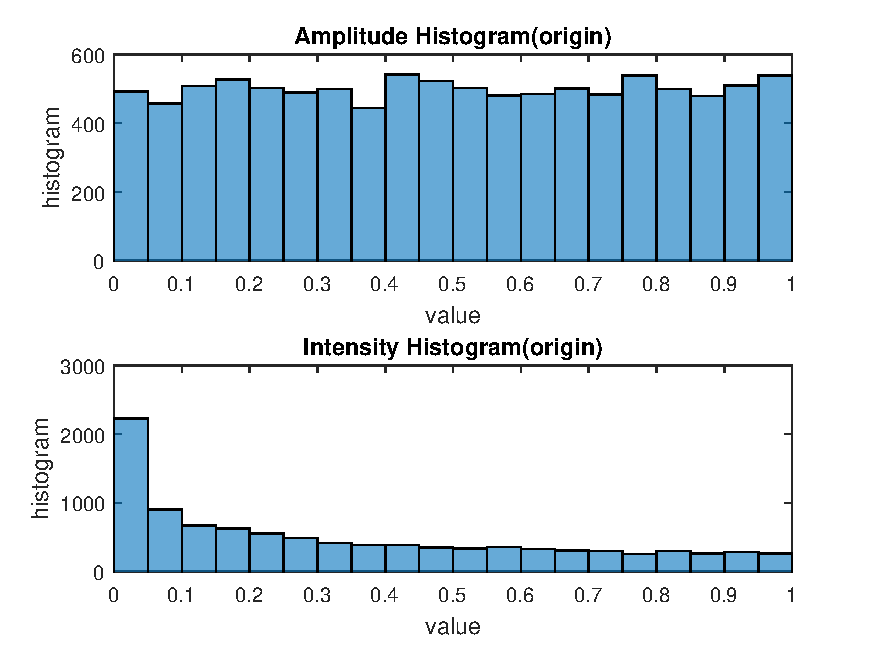
\includegraphics[width = 0.6\textwidth]{src/2pi/hist_origin.pdf}
	\caption{Histogram of amplitude (top) and intensity (bottom) of origin array}
	\label{fig:hist-origin}
\end{figure}
In Figure \ref{fig:hist-origin}, we can see the distribution of amplitude is exactly uniform distribution. Because intensity is $amplitude^2$ and 
value between [0, 1] will decay exponentially, so the distribution will move left.

\subsection{Histogram and Ratio of new array}
Now we create an new array with size \textbf{N (= 10000, 5000, 2000, 1000, 500)}, which value is the sum of \textbf{M (= 1, 2, 5, 10, 20)} consecutive data:
$$
	val(i) = \sum_{k = (i-1)*M}^{i*M}{origin(k)}
$$ 
And then plot their histogram and calculate ratio of mean and standard deviation as a function of M. 

Figure [\ref{fig:hist-500-20},   \ref{fig:hist-1000-10},  \ref{fig:hist-2000-5}, \ref{fig:hist-5000-2}, \ref{fig:hist-10000-1}] 
show the histogram result and Figure \ref{fig:ratio} show the ratio as a function of M.

\begin{figure}[H]
	\centering
	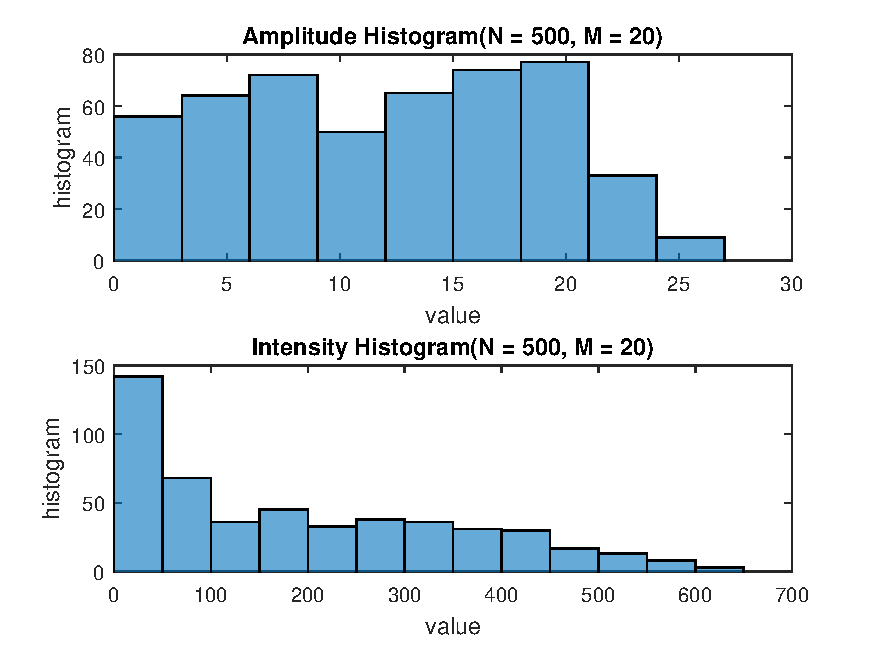
\includegraphics[width = 0.6\textwidth]{src/2pi/hist_500_20.pdf}
	\caption{Histogram of amplitude (top) and intensity (bottom) of new array (N = 500, M = 20)}
	\label{fig:hist-500-20}
\end{figure}
\begin{figure}[H]
	\centering
	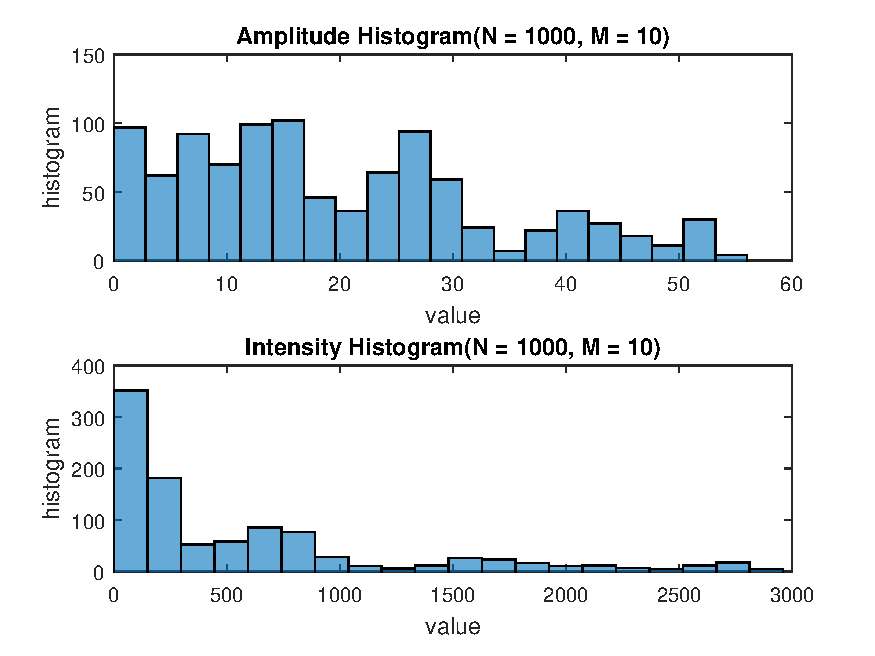
\includegraphics[width = 0.6\textwidth]{src/2pi/hist_1000_10.pdf}
	\caption{Histogram of amplitude (top) and intensity (bottom) of new array (N = 1000, M = 10)}
	\label{fig:hist-1000-10}
\end{figure}
\begin{figure}[H]
	\centering
	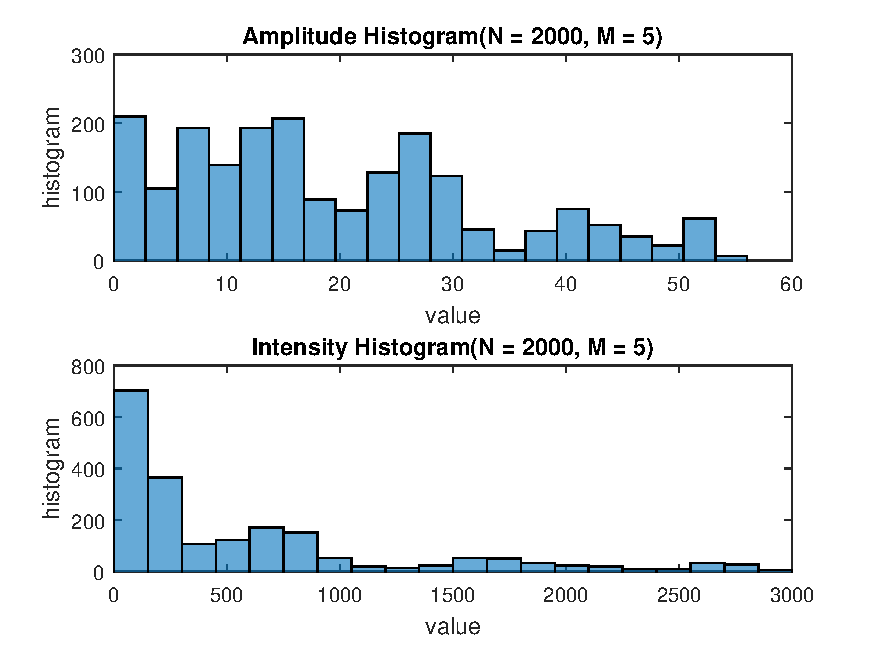
\includegraphics[width = 0.6\textwidth]{src/2pi/hist_2000_5.pdf}
	\caption{Histogram of amplitude (top) and intensity (bottom) of new array (N = 2000, M = 5)}
	\label{fig:hist-2000-5}
\end{figure}
\begin{figure}[H]
	\centering
	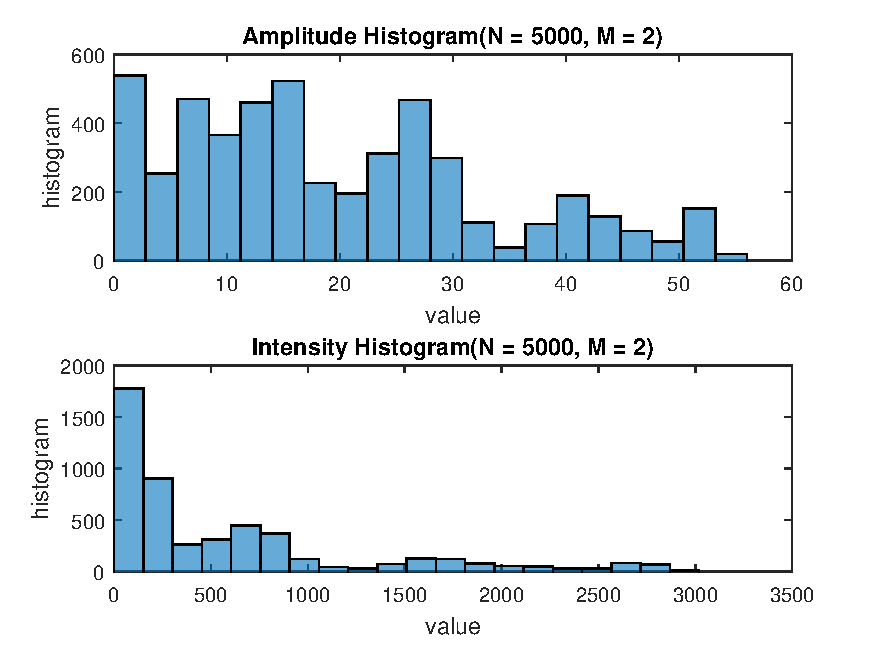
\includegraphics[width = 0.6\textwidth]{src/2pi/hist_5000_2.pdf}
	\caption{Histogram of amplitude (top) and intensity (bottom) of new array (N = 5000, M = 2)}
	\label{fig:hist-5000-2}
\end{figure}
\begin{figure}[H]
	\centering
	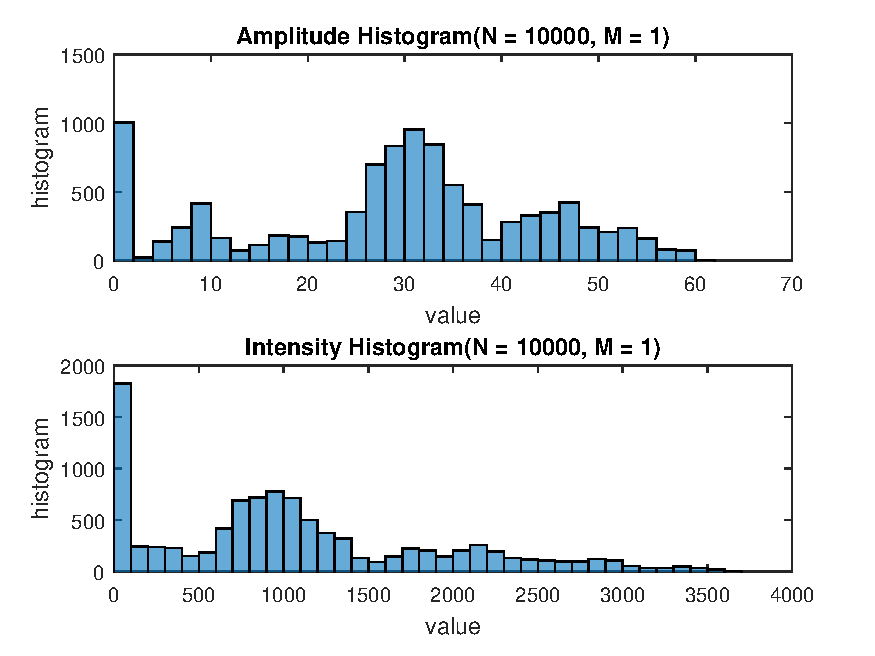
\includegraphics[width = 0.6\textwidth]{src/2pi/hist_10000_1.pdf}
	\caption{Histogram of amplitude (top) and intensity (bottom) of new array (N = 10000, M = 1)}
	\label{fig:hist-10000-1}
\end{figure}

\begin{figure}[H]
	\centering
	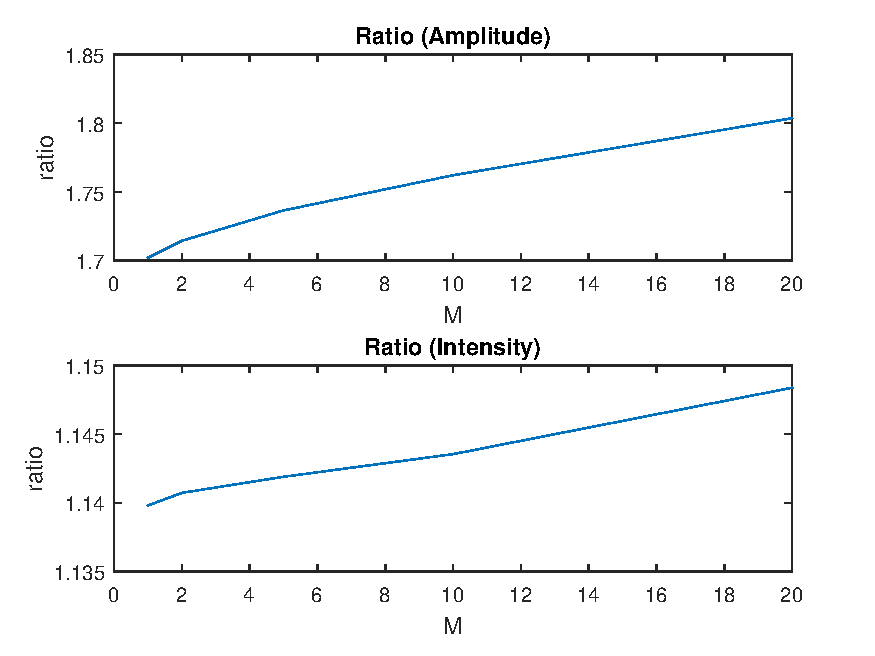
\includegraphics[width = 0.6\textwidth]{src/2pi/ratio.pdf}
	\caption{Ratio of mean and standard deviation}
	\label{fig:ratio}
\end{figure}


\subsection{Repeat (a) and (b) with phase distribution [0, $\pi$]}
Now we change the phase distribution of origin array from [0, $2\pi$] to [0, $\pi$]. Figure \ref{fig:hist-origin-pi} shows the histogram of 
amplitude and intensity of origin array with phase distribution [0, $\pi$]. 
Figure [\ref{fig:hist-500-20-pi}, \ref{fig:hist-1000-10-pi}, \ref{fig:hist-2000-5-pi}, \ref{fig:hist-5000-2-pi}, \ref{fig:hist-10000-1-pi}]
show histogram for different N and M.  Figure \ref{fig:ratio-pi} show the ratio.

\begin{figure}[H]
	\centering
	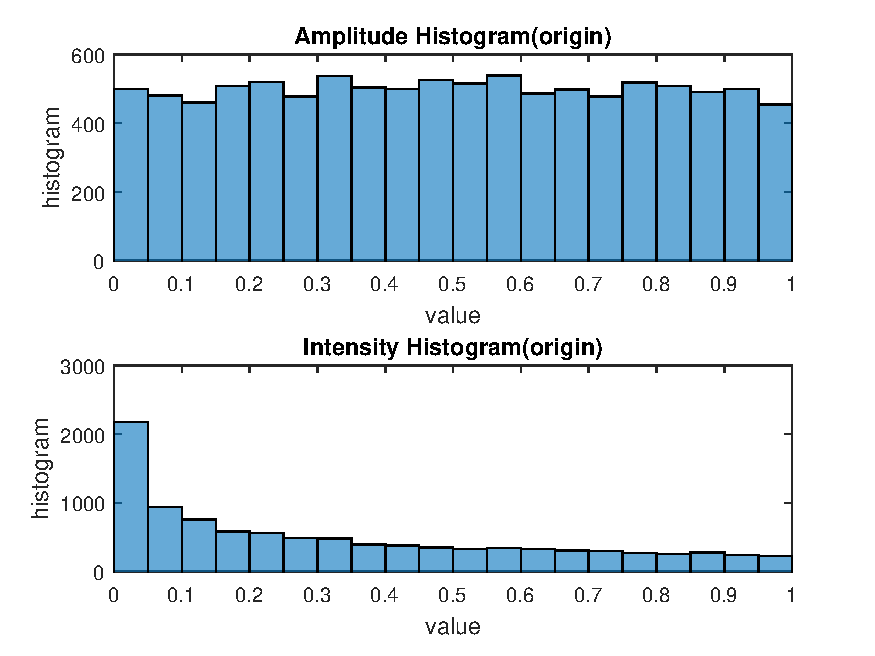
\includegraphics[width = 0.6\textwidth]{src/pi/hist_origin.pdf}
	\caption{Histogram of amplitude (top) and intensity (bottom) of origin array (phase = [0, $\pi$])}
	\label{fig:hist-origin-pi}
\end{figure}

\begin{figure}[H]
	\centering
	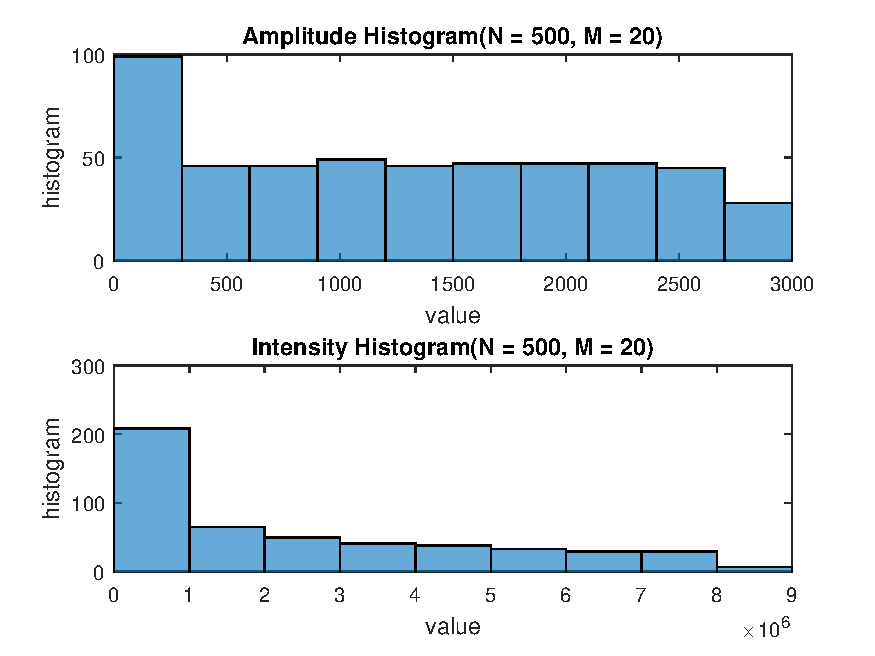
\includegraphics[width = 0.6\textwidth]{src/pi/hist_500_20.pdf}
	\caption{Histogram of amplitude (top) and intensity (bottom) of array (N = 500, M = 20, phase[0, $\pi$])}
	\label{fig:hist-500-20-pi}
\end{figure}
\begin{figure}[H]
	\centering
	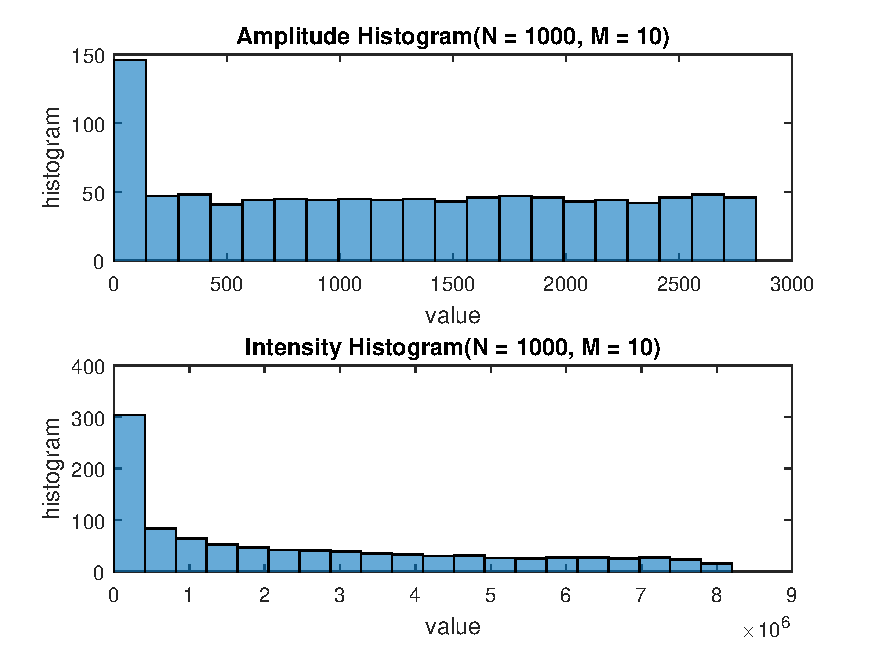
\includegraphics[width = 0.6\textwidth]{src/pi/hist_1000_10.pdf}
	\caption{Histogram of amplitude (top) and intensity (bottom) of array (N = 1000, M = 10, phase[0, $\pi$])}
	\label{fig:hist-1000-10-pi}
\end{figure}
\begin{figure}[H]
	\centering
	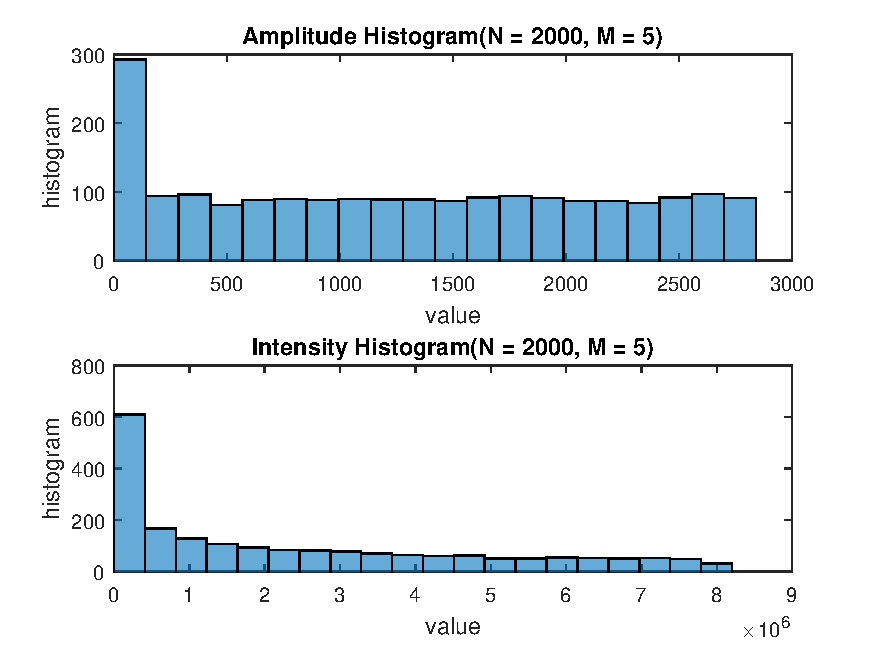
\includegraphics[width = 0.6\textwidth]{src/pi/hist_2000_5.pdf}
	\caption{Histogram of amplitude (top) and intensity (bottom) of array (N = 2000, M = 5, phase[0, $\pi$])}
	\label{fig:hist-2000-5-pi}
\end{figure}
\begin{figure}[H]
	\centering
	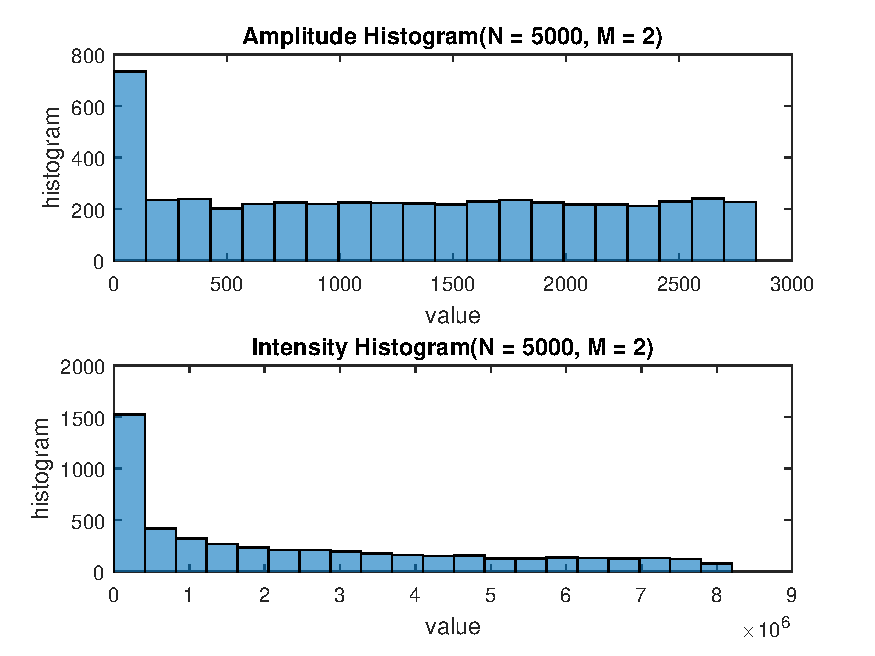
\includegraphics[width = 0.6\textwidth]{src/pi/hist_5000_2.pdf}
	\caption{Histogram of amplitude (top) and intensity (bottom) of array (N = 5000, M = 2, phase[0, $\pi$])}
	\label{fig:hist-5000-2-pi}
\end{figure}
\begin{figure}[H]
	\centering
	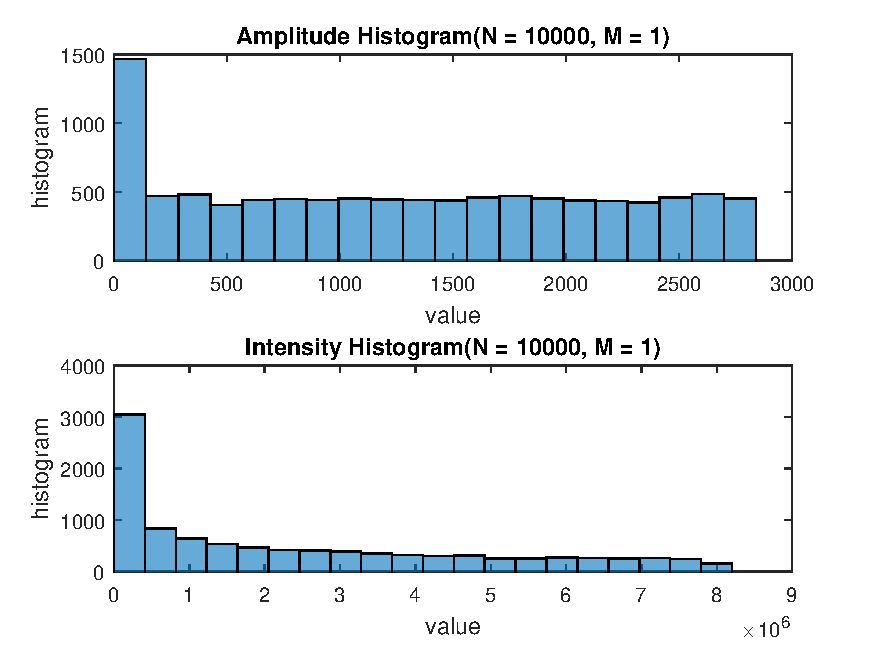
\includegraphics[width = 0.6\textwidth]{src/pi/hist_10000_1.pdf}
	\caption{Histogram of amplitude (top) and intensity (bottom) of array (N = 10000, M = 1, phase[0, $\pi$])}
	\label{fig:hist-10000-1-pi}
\end{figure}

\begin{figure}[H]
	\centering
	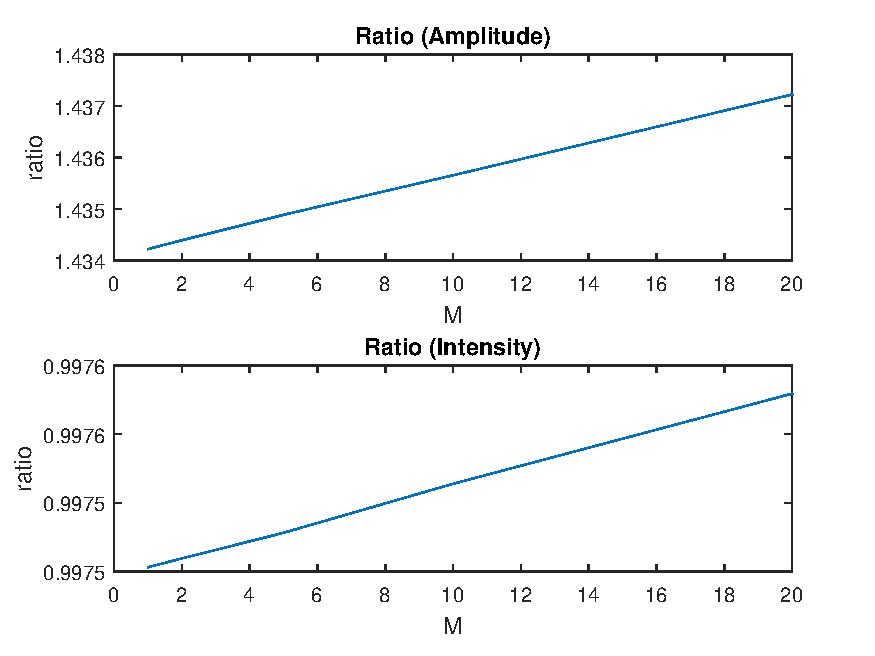
\includegraphics[width = 0.6\textwidth]{src/pi/ratio.pdf}
	\caption{Ratio of mean and standard deviation (phase[0, $\pi$])}
	\label{fig:ratio-pi}
\end{figure}


\subsection{Smooth amplitude and intensity}
Now we will use a moving average filter [0.5, 0.5] to smooth the amplitude and intensity, which is a post-processing. 
Figure \ref{fig:ratio_smooth_later} show the ratio as a function of M for different N.
\begin{figure}[H]
	\centering
	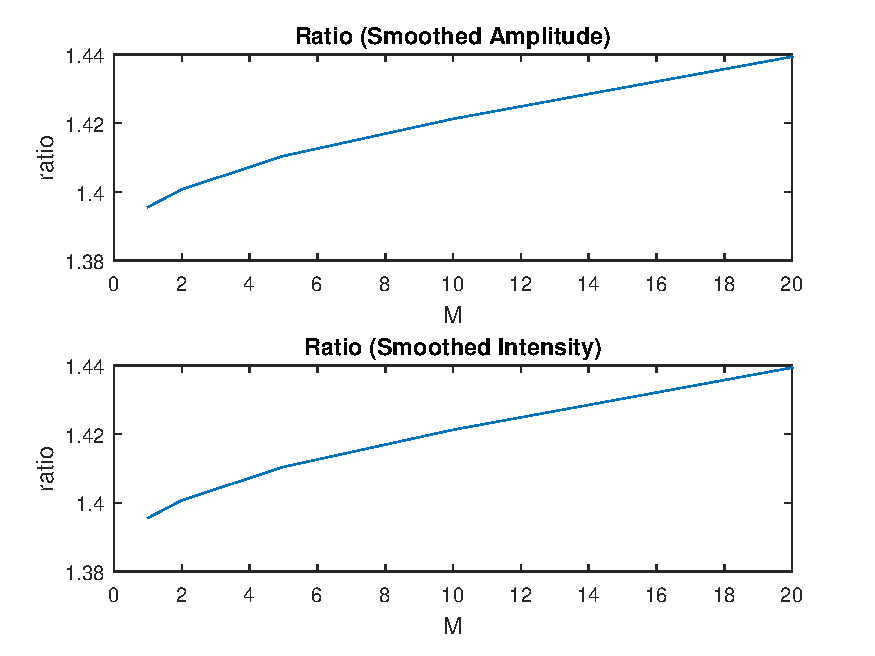
\includegraphics[width = 0.6\textwidth]{src/2pi/ratio_smooth_later.pdf}
	\caption{Ratio as function of M with smoothed amplitude and intensity}
	\label{fig:ratio_smooth_later}
\end{figure}

\subsection{Smooth new array}
Now we will try to use the same filter to smooth new array obtained from (b), which is a pre-processing.
Figure \ref{fig:ratio_smooth_first} show the ratio as a function of M for different N.
\begin{figure}[H]
	\centering
	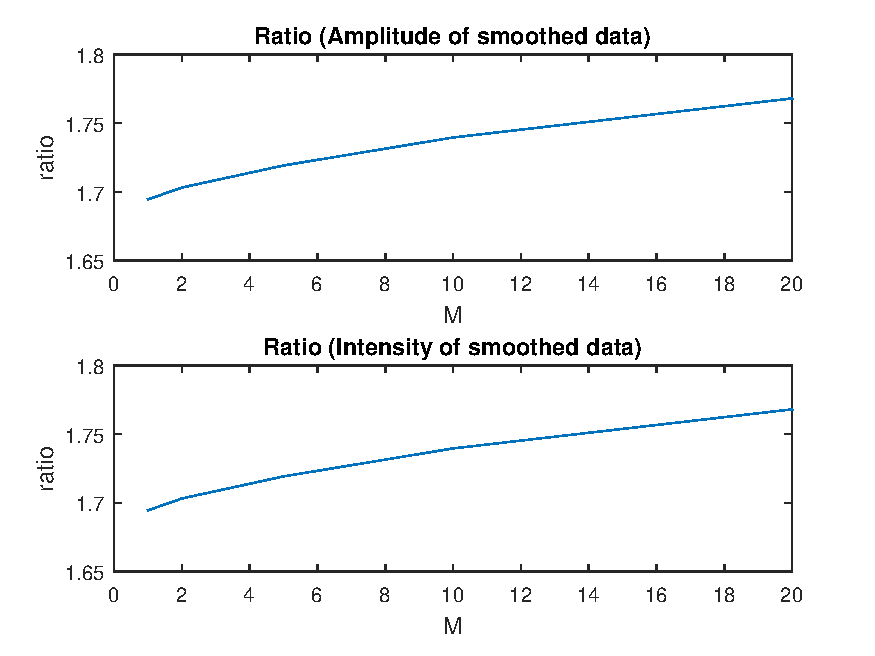
\includegraphics[width = 0.6\textwidth]{src/2pi/ratio_smooth_first.pdf}
	\caption{Ratio as function of M with smoothed data array}
	\label{fig:ratio_smooth_first}
\end{figure}

\section{Part \RN{2}}
In this part, we will use Matlab tool \textbf{Field2} to simulate phantom scattering.

\subsection{Ratio of two area}
Now we should calculate the ratio of mean to the standard deviation for amplitude and intensity. To divide the image into
two part, I manually crop 2 area from the image which one is lighter and the other is darker. The ratio is summarized as Table \ref{tab:ratio}:

\begin{table}[H]
  \centering
    \begin{tabular}{|c|c|c|}
    \hline
          & Experimental Ratio & Theoretical Ratio \bigstrut\\
    \hline
    Amplitude (higher scattering inclusion) &   1.6517    &  \bigstrut\\
    \hline
    Intensity (higher scattering inclusion) &   0.8688    &  \bigstrut\\
    \hline
    Amplitude (speckle background) &   1.7776    &  \bigstrut\\
    \hline
    Intensity (speckle background) &   0.8742    &  \bigstrut\\
    \hline
    \end{tabular}%
  \caption{Ratio for lighter/darker area}
  \label{tab:ratio}%
\end{table}%

\subsection{Contrast of two area}
For the two area, we will calculate their contrast by following formula:
$$
	contrast = \abs{I_1 - I_2}
$$
where $I_1$ and $I_2$ are mean value in dB. Table \ref{tab:contrast} show the result.
\begin{table}[H]
  \centering
  
    \begin{tabular}{|c|c|c|}
    \hline
          & Experimental Contrast & Theoretical Contrast \bigstrut\\
    \hline
    Amplitude & 16.9036 & 20 \bigstrut\\
    \hline
    Intensity & 33.8073 & 40 \bigstrut\\
    \hline
    \end{tabular}%
    \caption{Contrast of amplitude/intensity}
  \label{tab:contrast}%
\end{table}%
Because the contrast of intensity is $20 * \log(amplitude^2) = 2 * 20 log(amplitude)$, so the value should be double than amplitude.

\subsection{Reduce the contrast}
Reduce contrast value until we cannot tell which part is lighter or darker in image. Figure 
[\ref{fig:contrast-20}, \ref{fig:contrast-10}, \ref{fig:contrast-7}, \ref{fig:contrast-5}] show result of contrast [20, 10, 7, 5], respectively.
\begin{figure}[H]
	\centering
	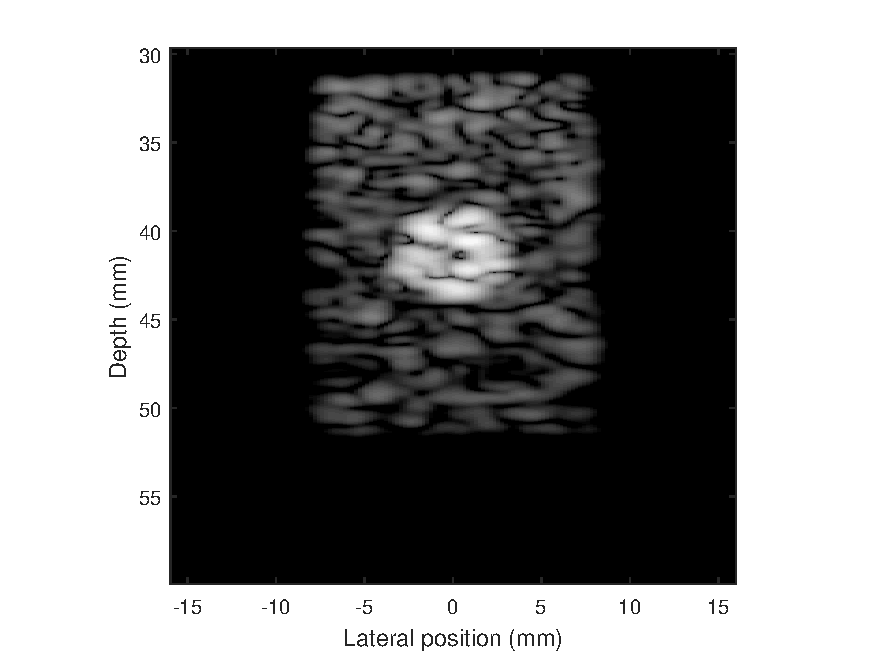
\includegraphics[width = 0.6\textwidth]{src/contrast_20.pdf}
	\caption{Contrast = 20}
	\label{fig:contrast-20}
\end{figure}
When contrast = 20 (Figure \ref{fig:contrast-20}), the border of lighter and darker area is clear to tell.
\begin{figure}[H]
	\centering
	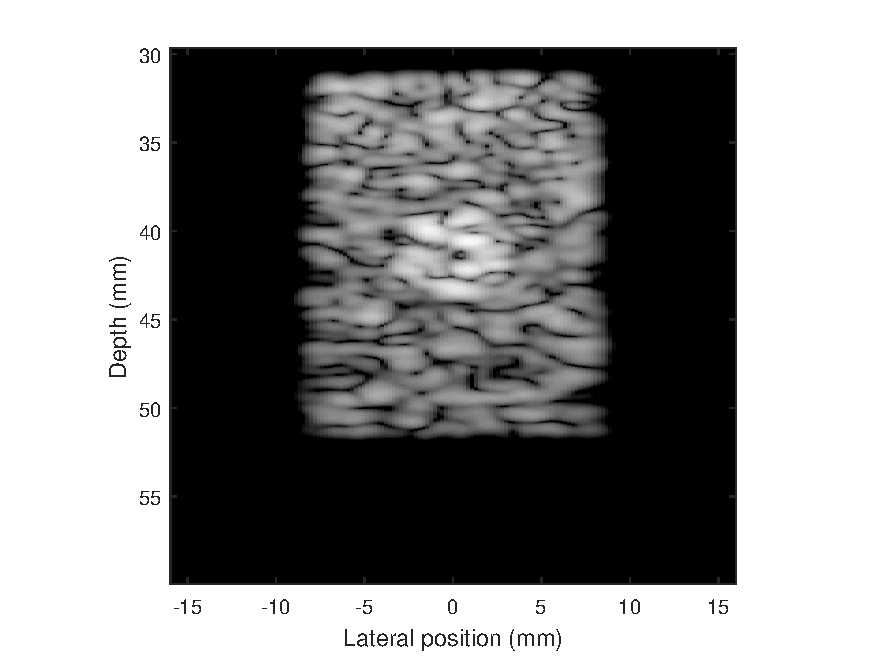
\includegraphics[width = 0.6\textwidth]{src/contrast_10.pdf}
	\caption{Contrast = 10}
	\label{fig:contrast-10}
\end{figure}
When contrast = 10 (Figure \ref{fig:contrast-10}), the intensity of two area is close but we can see the border clearly.
\begin{figure}[H]
	\centering
	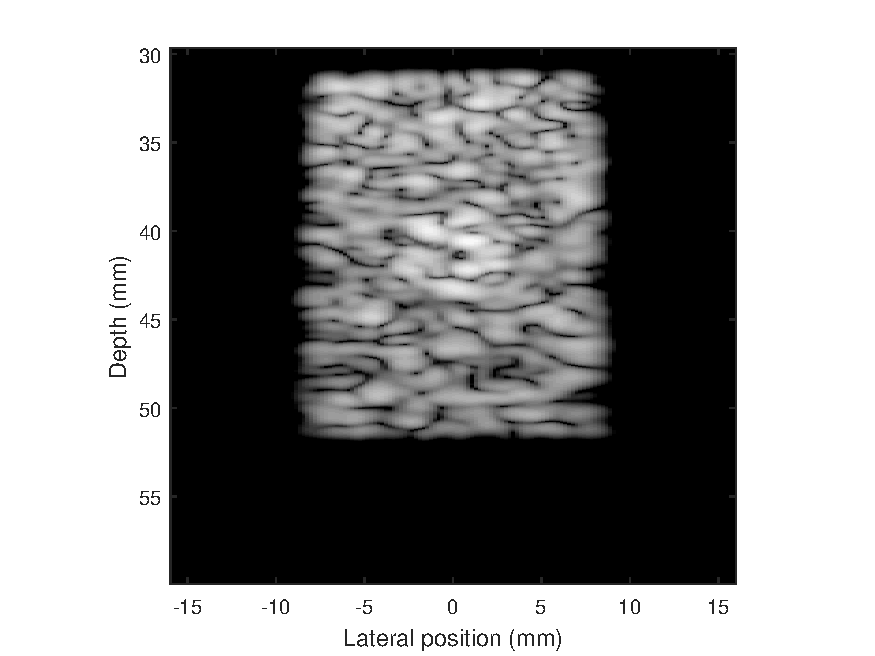
\includegraphics[width = 0.6\textwidth]{src/contrast_7.pdf}
	\caption{Contrast = 7}
	\label{fig:contrast-7}
\end{figure}
When contrast = 7 (Figure \ref{fig:contrast-7}), the intensity of two area is very close and border is very unclear.
\begin{figure}[H]
	\centering
	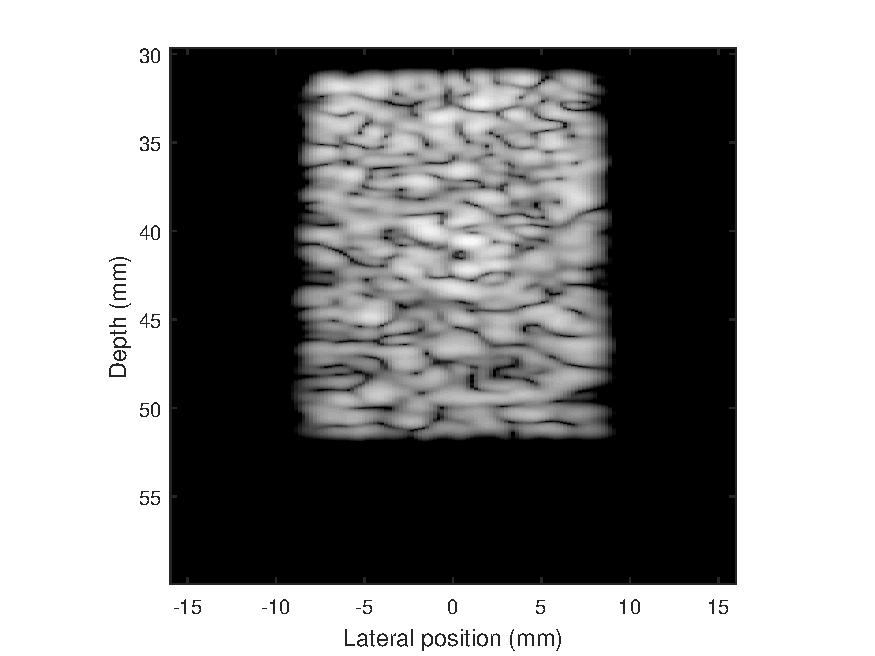
\includegraphics[width = 0.6\textwidth]{src/contrast_5.pdf}
	\caption{Contrast = 5}
	\label{fig:contrast-5}
\end{figure}
When contrast = 5 (Figure \ref{fig:contrast-5}), the border totally disappear.

As a result, I think the \textbf{minimum detectable contrast is 7 dB}.

\end{document}















